% $Header: /home/vedranm/bitbucket/beamer/solutions/generic-talks/generic-ornate-15min-45min.en.tex,v 90e850259b8b 2007/01/28 20:48:30 tantau $

\documentclass{beamer}
  
% This file is a solution template for:

% - Giving a talk on some subject.
% - The talk is between 15min and 45min long.
% - Style is ornate.



% Copyright 2004 by Till Tantau <tantau@users.sourceforge.net>.
%
% In principle, this file can be redistributed and/or modified under
% the terms of the GNU Public License, version 2.
%
% However, this file is supposed to be a template to be modified
% for your own needs. For this reason, if you use this file as a
% template and not specifically distribute it as part of a another
% package/program, I grant the extra permission to freely copy and
% modify this file as you see fit and even to delete this copyright
% notice. 


\mode<presentation>
{
  \usetheme{Marburg}
  \usecolortheme{beaver}

  \setbeamercovered{transparent}
  % or whatever (possibly just delete it)
}
\usepackage{amsmath}

\usepackage[english]{babel}
% or whatever

\usepackage[latin1]{inputenc}
% or whatever

\usepackage{times}
\usepackage[T1]{fontenc}
% Or whatever. Note that the encoding and the font should match. If T1
% does not look nice, try deleting the line with the fontenc.


\title[Governing Equations] % (optional, use only with long paper titles)
{Governing Equations of Classical Gas Dynamics}

\subtitle
{From Euler form to the Characteristics form} % (optional)

\author[Manuel Diaz] % (optional, use only with lots of authors)
{Manuel Diaz\inst{1} }
% - Use the \inst{?} command only if the authors have different
%   affiliation.

\institute[National Taiwan University] % (optional, but mostly needed)
{
  \inst{1}%
  National Taiwan University\\
  Institute of Applied Mechanics}
%  \and
%  \inst{2}%
%  Department of Theoretical Philosophy\\
%  University of Elsewhere}
% - Use the \inst command only if there are several affiliations.
% - Keep it simple, no one is interested in your street address.

\date[August 31th, 2011] % (optional)
{August 31th, 2011 / Weekly Meeting}

\subject{Talks}
% This is only inserted into the PDF information catalog. Can be left
% out. 



% If you have a file called "university-logo-filename.xxx", where xxx
% is a graphic format that can be processed by latex or pdflatex,
% resp., then you can add a logo as follows:

% \pgfdeclareimage[height=0.5cm]{university-logo}{university-logo-filename}
% \logo{\pgfuseimage{university-logo}}



% Delete this, if you do not want the table of contents to pop up at
% the beginning of each subsection:
\AtBeginSubsection[]
{
  \begin{frame}<beamer>{Outline}
    \tableofcontents[currentsection,currentsubsection]
  \end{frame}
}


% If you wish to uncover everything in a step-wise fashion, uncomment
% the following command: 

%\beamerdefaultoverlayspecification{<+->}


\begin{document}

\begin{frame}
  \titlepage
\end{frame}

\begin{frame}{Outline}
  \tableofcontents
  % You might wish to add the option [pausesections]
\end{frame}


% Since this a solution template for a generic talk, very little can
% be said about how it should be structured. However, the talk length
% of between 15min and 45min and the theme suggest that you stick to
% the following rules:  

% - Exactly two or three sections (other than the summary).
% - At *most* three subsections per section.
% - Talk about 30s to 2min per frame. So there should be between about
%   15 and 30 frames, all told.

\section{Introduction: Euler Equations}

\subsection[Integral and Conservation form]{Integral and Conservation form}

\begin{frame}{INTEGRAL FORM}
  Conservation of Mass: ``All mass in the universe is constant''
  \begin{figure}
    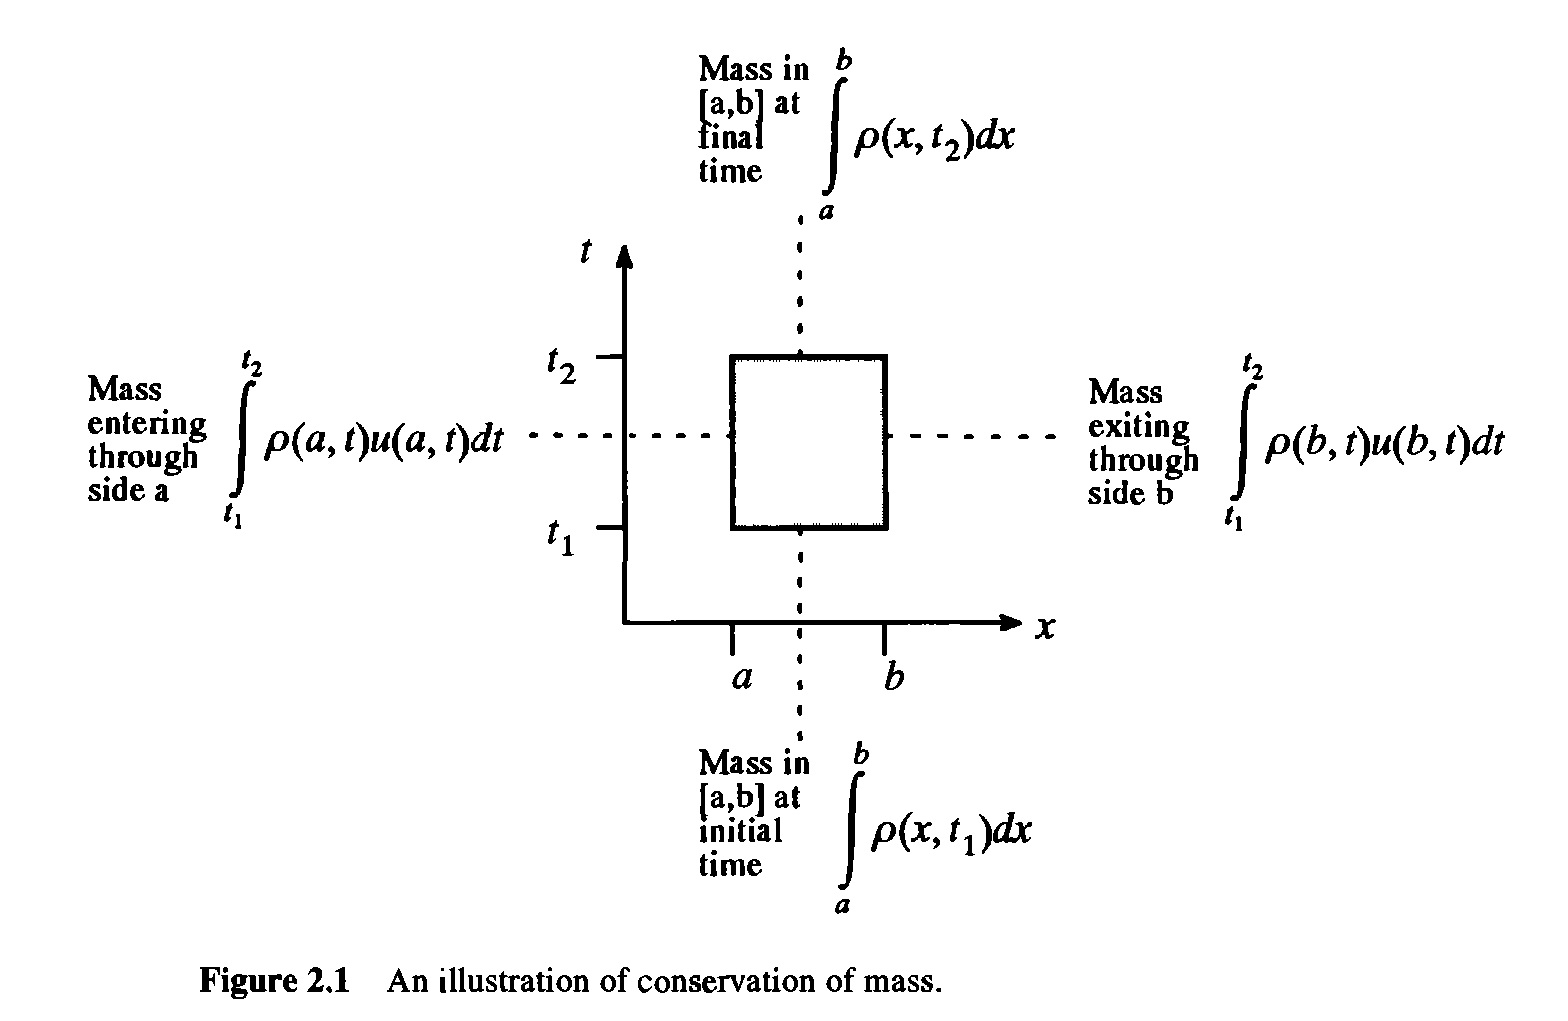
\includegraphics[scale=.17]{figures/MassConservation.jpg}
  \end{figure}
    In a space-time \texttt{(x,t)} plane a control volume is depicted.
\end{frame}
 

\begin{frame}{INTEGRAL FORM}{for mass}
  Change in total mass in \texttt{[a,b]} in time interval \texttt{[$t_1$,$t_2$]} = net mass passing through boundaries of \texttt{[a,b]} in time interval \texttt{[$t_1$,$t_2$]}.
  \begin{eqnarray}\nonumber
    && \int\limits_a^b[\rho(x,t_2)-\rho(x,t_1)dx = \nonumber \\
    && -\int\limits_{t_1}^{t_2}[\rho(b,t)u(b,t)-\rho(a,t)u(a,t)]dt
  \end{eqnarray}
\end{frame}

\begin{frame}{INTEGRAL FORM}{for momentum}
  Change in total momentum in \texttt{[a,b]} in time interval \texttt{[$t_1$,$t_2$]} = net momentum passing through boundaries of \texttt{[a,b]} in time interval \texttt{[$t_1$,$t_2$]} + net momentum change due to pressure on boundaries of \texttt{[a,b]}.
  \begin{eqnarray}
    && \int\limits_a^b[\rho(x,t_2)u(x,t_2)-\rho(x,t_1)u(x,t_1)]dx = \nonumber \\
    && -\int\limits_{t_1}^{t_2}[\rho(b,t)u^2(b,t)-\rho(a,t)u^2(a,t)]dt \nonumber \\
    && -\int\limits_{t_1}^{t_2}[p(b,t)-p(a,t)]dt 
  \end{eqnarray}
\end{frame}

\begin{frame}{INTEGRAL FORM}{for Energy}
  Change in total Energy in \texttt{[a,b]} in time interval \texttt{[$t_1$,$t_2$]} = net Energy passing through boundaries of \texttt{[a,b]} in time interval \texttt{[$t_1$,$t_2$]} + net Energy change due to pressure on boundaries of \texttt{[a,b]}.
  \begin{eqnarray}\nonumber
    && \int\limits_a^b[\rho(x,t_2)e_T(x,t_2)-\rho(x,t_1)e_T(x,t_1)]dx = \nonumber \\
    && -\int\limits_{t_1}^{t_2}[\rho(b,t)u(b,t)e_T(b,t)-\rho(a,t)u(a,t)e_T(b,t)]dt \nonumber \\
    && -\int\limits_{t_1}^{t_2}[p(b,t)u(b,t)-p(b,t)u(b,t)]dt 
  \end{eqnarray}
\end{frame}

\begin{frame}{INTEGRAL FORM}{Entropy and 2nd Law}
  By 2nd Law of Thermodynamics we know: The total entropy of the universe never decreases.
  \begin{itemize}
   \item how is Entropy defined for an Ideal Gas?
  \end{itemize}
  \begin{eqnarray}
    &&{\Delta}S=\int\limits_{T_0}^T \frac{Cv}{T}dT+\int\limits_{V_0}^{V} \left(\frac{\partial{p}}{\partial{T}}\right)_VdV \nonumber \\
    &&{\Delta}S=C_vNkln\left(\frac{T}{T_0}\right)+Nkln\left(\frac{V}{V_0}\right)\nonumber \\
    &&{\Delta}S=C_vNkln(T)+Nkln(V) \nonumber
  \end{eqnarray}
\end{frame}

\begin{frame}{INTEGRAL FORM}{Ideal Gas relations}
  \begin{itemize}
   \item Ideal gas equation of state:
  \end{itemize}
  \begin{eqnarray}
    && p={\rho}RT \nonumber \\
    && e = c_v T \nonumber \\
    && h = c_p T \nonumber \\
    && \gamma = \frac{c_p}{c_v} \nonumber \\
    && c_p = R + c_v \nonumber 
  \end{eqnarray}
\end{frame}

\begin{frame}{INTEGRAL FORM}{Entropy and 2nd Law}
   \begin{itemize}
   \item the equation of state giving specific entropy \texttt{s} as a fuction of specific internal energy and density:
  \end{itemize}
  \begin{eqnarray}\nonumber
    && s=c_vlne-Rln\rho+const. \\
    && s=c_vlnp-c_pln\rho+const.
  \end{eqnarray}
\end{frame}

\begin{frame}{INTEGRAL FORM}{Entropy and 2nd Law}
   \begin{itemize}
   \item for homentropic conditions, we conclude:
  \end{itemize}
  \begin{eqnarray}\nonumber
    && p=(const.)\rho^\gamma \nonumber \\
    && T=(const.)\rho^{\gamma-1} \nonumber  \\
    && a=(const.)\rho^{(\gamma-1)/2} \nonumber 
  \end{eqnarray}
\end{frame}

\begin{frame}{INTEGRAL FORM}{Entropy and 2nd Law}
  The change in total entropy in \texttt{[a,b]} in time interval \texttt{[$t_1$,$t_2$]} $\geq$ net entropy passing through boundaries of \texttt{[a,b]} in time interval \texttt{[$t_1$,$t_2$]}.
  \begin{eqnarray}\nonumber
    && \int\limits_a^b[\rho(x,t_2)s(x,t_2)-\rho(x,t_1)s(x,t_1)]dx \geq \nonumber \\
    && -\int\limits_{t_1}^{t_2}[\rho(b,t)u(b,t)s(b,t)-\rho(a,t)u(a,t)s(b,t)]dt
  \end{eqnarray}
\end{frame}

\begin{frame}{CONSERVATION FORM}{Vector Notation}
  \begin{itemize}
   \item Define the Vectors of conserved quantities:
  \end{itemize}
  \begin{equation}
    \vec{u} = \begin{bmatrix}
      {\rho} \\
      {\rho}{u} \\
      {\rho}{e_T}
    \end{bmatrix}=\begin{bmatrix}
      u_1\\ 
      u_2\\ 
      u_3
      \end{bmatrix}
  \end{equation}
  \begin{equation}
   \vec{f} = \begin{bmatrix}
      {\rho}{u} \\
      {\rho}{u^2}+p \\
      ({\rho}{e_T}+p)u
    \end{bmatrix}=\begin{bmatrix}
      f_1\\ 
      f_2\\ 
      f_3
      \end{bmatrix}
  \end{equation}
\end{frame}

\begin{frame}{CONSERVATION FORM}
  \begin{itemize}
   \item We can rewrite more compactly the conservation equations 1 to 3:
  \end{itemize}
  \begin{equation}
   \int\limits_a^b[\vec{u}(x,t_2)-\vec{u}(x,t_1)dx = -\int\limits_{t_1}^{t_2}[\vec{f}(b,t)-\vec{f}(a,t)dx
  \end{equation}
\end{frame}

\begin{frame}{CONSERVATION FORM}
  \begin{itemize}
   \item Take the mass integral conservation (Ec.1)
   \item Asume that $\rho(x,t)$ is differentiable in time. 
   \item Using the fundamental theorem of calculus we can rewrite:
  \end{itemize}
  \begin{equation}
    {\rho}(x,t_2)-{\rho}(x,t_1)=\int\limits_{t_1}^{t_2} \frac{\partial{\rho}}{\partial{t}}dt
  \end{equation}
\end{frame}

\begin{frame}{CONSERVATION FORM}
  \begin{itemize}
   \item Similarly, if $\rho(x,t)u(x,t)$ is diffentiable in space the we can rewrite:
  \end{itemize}
  \begin{equation}
    {\rho}(b,t)u(b,t)-{\rho}(a,t)u(a,t)=\int\limits_a^b \frac{\partial{{\rho}{u}}}{\partial{t}}dt
  \end{equation}
\end{frame}

\begin{frame}{CONSERVATION FORM}
  \begin{itemize}
   \item Assuming integration in space is reversible with integration in time, Ec. 1 becomes:
  \end{itemize}
  \begin{equation}
    \int\limits_a^b \int\limits_{t_1}^{t_2} \left[ \frac{\partial{\rho}}{\partial{t}} +\frac{\partial{{\rho}{u}}}{\partial{x}} \right] dtdx = 0
  \end{equation} 
\end{frame}

\begin{frame}{CONSERVATION FORM}
  \begin{itemize}
   \item The conservation form of the Euler Equations:
  \end{itemize}
  \begin{eqnarray}
    &&\frac{\partial{\rho}}{\partial{t}}+\frac{\partial{{\rho}{u}}}{\partial{x}}=0, \\
    &&\frac{\partial{{\rho}u}}{\partial{t}}+\frac{\partial{({\rho}{u^2}+p})}{\partial{x}}=0, \\
    &&\frac{\partial{\rho}e_T}{\partial{t}}+\frac{\partial{({\rho}{u}e_T+pu})}{\partial{x}}=0, \\
    &&\frac{\partial{\rho}s}{\partial{t}}+\frac{\partial{{\rho}{u}s}}{\partial{x}}=0.
  \end{eqnarray} 
\end{frame}

\subsection{Vector-Matrix Notation}
  
\begin{frame}{VECTOR NOTATION}
  \begin{itemize}
   \item Using againg the vector notation the conservation equation can be written as:
  \end{itemize}
  \begin{equation}
   \frac{\partial{\vec{u}}}{\partial{t}}+\frac{\partial{\vec{f}}}{\partial{x}}=0
  \end{equation}
\end{frame}

\begin{frame}{VECTOR NOTATION}
  \begin{itemize}
   \item The by the chain rule
  \end{itemize}
  \begin{equation}
   \frac{\partial{\vec{u}}}{\partial{x}}=\frac{d\vec{f}}{d\vec{u}}\frac{\partial{\vec{u}}}{\partial{x}}
  \end{equation}
  where
  \begin{equation}
    \frac{\partial{\vec{u}}}{\partial{x}}=\begin{bmatrix}
    \frac{\partial{f_1}}{\partial{u_1}} & \frac{\partial{f_1}}{\partial{u_2}} & \frac{\partial{f_1}}{\partial{u_3}}\\ 
    \frac{\partial{f_2}}{\partial{u_1}} & \frac{\partial{f_2}}{\partial{u_2}} & \frac{\partial{f_2}}{\partial{u_3}}\\ 
    \frac{\partial{f_3}}{\partial{u_1}} & \frac{\partial{f_3}}{\partial{u_2}} & \frac{\partial{f_3}}{\partial{u_3}}
    \end{bmatrix}
  \end{equation}
\end{frame}

\begin{frame}{MATRIX NOTATION}
  \begin{itemize}
   \item To simplify, we call the Jacobian Matrix: A
  \end{itemize}
  \begin{equation}
    \frac{\partial{\vec{u}}}{\partial{t}}+A\frac{\partial{\vec{u}}}{\partial{x}}=0
  \end{equation}
  Computing A we obtain:
  \begin{equation}
   A=\begin{bmatrix}
    0 & 1 & 0\\ 
    \frac{\gamma-3}{2}u^2 & (3-\gamma)u & \gamma-1\\ 
    {\gamma}{u}e_T+(\gamma-1)u^3 & {\gamma}e_T-\frac{3}{2}(\gamma-1)u^2 & {\gamma}u
    \end{bmatrix}
  \end{equation}
\end{frame}

\subsection{Primitive Variable Form}

\begin{frame}{THE MATERIAL}
  \begin{itemize}
   \item The Primite variable from is not commonly used in gasdynamics. 
   \item The Primite variables are those flow variable that we can dyrectly measure.
   \item This is a lagrangean description of the variables.
  \end{itemize}
The Material Derivate:
  \begin{equation}
   \frac{D}{Dt}=\frac{\partial}{\partial{t}}+u\frac{\partial}{\partial{x}}
  \end{equation}
\end{frame}

\begin{frame}{LAGRANGE EQUATIONS}
  \begin{itemize}
   \item The material derivate is rate of change a long the pathlines.
   \item Using the material derivate we rewrite the Euler Equations as:
  \end{itemize}
The Material Derivate:
  \begin{eqnarray}
    &&\frac{D\rho}{Dt}+\rho\frac{\partial{u}}{\partial{x}}=0 \\
    &&\frac{D\rho}{Dt}+\frac{1}{\rho}\frac{\partial{p}}{\partial{x}}=0 \\
    &&\frac{D\rho}{Dt}+{\rho}a^2\frac{\partial{u}}{\partial{x}}=0 \\
    &&\frac{Ds}{Dt}\geq 0
  \end{eqnarray}
\end{frame}

\begin{frame}{VECTOR-MATRIX FORM}
  \begin{itemize}
   \item Define the vector of primitive variables:
  \end{itemize}
The Material Derivate:
  \begin{equation}
   \vec{w}=\begin{bmatrix}
   \rho\\ 
   u\\ 
   p
   \end{bmatrix}
  \end{equation}
\end{frame}

\begin{frame}{VECTOR-MATRIX FORM}
  \begin{itemize}
   \item Then primitive form of the Euler equations can be written as:
  \end{itemize}
  \begin{equation}
   \frac{\partial{\vec{w}}}{\partial{t}}+C\frac{\partial{\vec{w}}}{\partial{x}}=0
  \end{equation}
Where:
  \begin{equation}
   C=\begin{bmatrix}
    u & \rho & 0\\ 
    0 & u & \frac{1}{\rho}\\ 
    0 & {\rho}a^2 & u
    \end{bmatrix}
  \end{equation}
\end{frame}

\begin{frame}{IMPORTANT RELATIONS}
  \begin{itemize}
   \item Relations between A and C: First notice that:
  \end{itemize}
  \begin{equation}
    d\vec{u}=Qd\vec{w}
  \end{equation}
where
  \begin{equation}
    Q=\frac{d\vec{u}}{d\vec{w}}=\begin{bmatrix}
    1 & 0 & 0\\ 
    u & \rho & 0\\ 
    \frac{1}{2}u^2 & {\rho}u & \frac{1}{\gamma-1}
    \end{bmatrix} 
  \end{equation}
\end{frame}

\begin{frame}{IMPORTANT RELATIONS}
  \begin{itemize}
   \item Relations between A and C: Or:
  \end{itemize}
  \begin{equation}
    d\vec{w}=Qd^{-1}\vec{u} 
  \end{equation}
where
  \begin{equation}
    Q^{-1}=\frac{d\vec{w}}{d\vec{u}}=\begin{bmatrix}
    1 & 0 & 0\\ 
    -\frac{1}{\rho}u & \frac{1}{\rho} & 0\\ 
    1/2(\rho-1)u^2 & -(\rho-1)u & \gamma-1
    \end{bmatrix}
  \end{equation}
\end{frame}

\begin{frame}{IMPORTANT RELATIONS}
  \begin{itemize}
   \item Relations between A and C:
  \end{itemize}
  \begin{eqnarray}
   &&Q\frac{\partial{\vec{w}}}{\partial{t}}+AQ\frac{\partial{\vec{w}}}{\partial{x}}=0 \\
   &&\frac{\partial{\vec{w}}}{\partial{t}}+Q^{-1}AQ\frac{\partial{\vec{w}}}{\partial{x}}=0 \\
   &&\frac{\partial{\vec{w}}}{\partial{t}}+C\frac{\partial{\vec{w}}}{\partial{x}}=0
  \end{eqnarray}
  \begin{itemize}
   \item In other words, A and C are similar matrices!
  \end{itemize}
\end{frame}

\section{Wave Models}

\subsection{Scalar Wave Model}

\begin{frame}{TITLE}
\end{frame}

\begin{frame}{TITLE}
\end{frame}

\subsection{Vector Wave Model}

\begin{frame}{TITLE}
\end{frame}

\begin{frame}{TITLE}
\end{frame}

\subsection{The Characteristic Form}

\begin{frame}{TITLE}
\end{frame}

\begin{frame}{TITLE}
\end{frame}

\section{Simple Waves}

\subsection{Isotropic Flow}

\begin{frame}{TITLE}
\end{frame}

\begin{frame}{TITLE}
\end{frame}

\subsection{Expansion Waves}

\begin{frame}{TITLE}
\end{frame}

\begin{frame}{TITLE}
\end{frame}

\subsection{Compresion Waves/Shock Waves}

\begin{frame}{TITLE}
\end{frame}

\begin{frame}{TITLE}
\end{frame}

\subsection{Contact Discontinuities}

\begin{frame}{TITLE}
\end{frame}

\begin{frame}{TITLE}
\end{frame}

\section*{Summary}

\begin{frame}{Summary}

  % Keep the summary *very short*.
  \begin{itemize}
  \item
    The \alert{first main message} of your talk in one or two lines.
  \item
    The \alert{second main message} of your talk in one or two lines.
  \item
    Perhaps a \alert{third message}, but not more than that.
  \end{itemize}
  
  % The following outlook is optional.
  \vskip0pt plus.5fill
  \begin{itemize}
  \item
    Outlook
    \begin{itemize}
    \item
      Something you haven't solved.
    \item
      Something else you haven't solved.
    \end{itemize}
  \end{itemize}
\end{frame}


\end{document}


